
\documentclass[a4paper,10pt]{article}
\usepackage{epsfig}
\usepackage{latexsym}
\usepackage{graphicx}
\usepackage{amsfonts}
\usepackage{amsmath}
\usepackage{xcolor}
\usepackage[utf8]{inputenc}   % LaTeX, comprends les accents !
\usepackage[T1]{fontenc}      % Police contenant les caractères français
\usepackage{geometry}         % Définir les marges
\usepackage[english]{babel}  % Placez ici une liste de langues, la
                              % dernière étant la langue principale        % Inserer des images
\usepackage{subfigure}
\usepackage{multicol}
\usepackage{caption}
\captionsetup{textfont=sl}
\usepackage{gensymb}
\usepackage{color}
\pagestyle{headings}          % Pour mettre des entêtes avec les titres
                              % des sections en haut de page

\title{\bf NIKA AHWP characterization}           % Les paramètres du titre : titre, auteur, date
\author{{\it Alessia Ritacco and the NIKA collaboration}}
\date{\today}

\setlength{\textwidth}{15.5cm}
\setlength{\textheight}{23cm}
\oddsidemargin +0.5cm                                          
\evensidemargin +0.5cm
\topmargin +0cm

\begin{document}

\maketitle                    
                              
\begin{figure}[!h]
\centering

\includegraphics[height=2cm,trim=0cm 0.1cm 0.1cm 0.1cm, clip=true]{figures/nika_white_bg}
\end{figure}
\vspace*{0.5cm}

\setcounter{page}{1}
\setcounter{tocdepth}{1}

\begin{abstract}
	From the previous characterization of the mono-chromatic HWP used during the campaign on January we found a source of polarization added to the signal probably due to the HWP itself. The transmission coefficients of the HWP were different in the two axis, this caused an incorrect functioning of the HWP that acted like a bad polarizing wire-grid.  the dedicated document for the details on the svn processing: \\($path$/url:{$home/Processing/Papers\_Proposal\_Notes/Reports/NIKAPol$}).
	The purpose of this document is to report the results of the tests effectuated to the "Institut NÉEL" laboratory in order to characterize the new achromatic half wave plate used during the campaign on October 2014.
	Another goal was measuring the effective optical axis in order to have a reference.
\end{abstract}

\section{Introduction}
A monochromatic wave plate can be simply obtained with a single slab of uniaxial birefringent crystal of specific thickness, which depends upon the wavelength and the index of refraction of the crystal. 
A birefringent crystal is characterized by four parameters, {$n_e$}, {$n_o$}, {$\alpha_e$}, {$\alpha_o$}, the real part of the indexes of refraction and absorption coefficient for the extraordinary and ordinary axes of the crystal.
At a specific wavelength {$\lambda_0$}, the phase shift induced by a slab is determined uniquely by its thickness d, and reads:
	
				\begin{equation}
				\Delta \phi (\lambda_0) =\frac{2 \pi  d ( n_e - n_o )}{ \lambda_0 }.
				\end{equation}
				
Given the operating wavelength {$\lambda_0$}, the required phase shift for the wave plate is achieved by tuning thickness d.
The dependence of the phase shift on wavelength, expressed in equation 1, constitutes an intrinsic limit in designing an HWP that operates in a broad spectral range. For this purpose is necessary to use an achromatic HWP (AHWP).
Multiple-slab solutions have been conceived to compensate and keep the phase shift approximately constant across the bandwidth, by stacking an odd number of birefringent substrates of the same material, which are rotated with respect to each other about their optical axes by a frequency-dependent set of angles.
				
\section{Measurements}
The tests have been done after the campaign, on October 2014. The subsections following detail the setup used in laboratory and the results of the measurements.
\subsection{Instrumental set-up}
We performed the spectral measurements using a Martin-Puplett interferometer and the AHWP placed and fixed in its mechanical modulator. For these tests we used one kids matrix with a frequency range a little bit narrow of NIKA bands, the signal incoming in the cryostat arrives on this one by reflection due to the polarizer mounted into the cryostat and cold at 100 mK.
The Martin-Puplett produces the difference between the powers of two input polarized beams which are built by two black bodies at different temperatures (ambient eccosorb and warmed eccosorb) modulated by a rotating wire-grid. The scan performed has a spectral resolution of about 3.5GHz (about 44 mm of excursion of the roof mirror) with a step of the roof mirror of 250{$\mu$}m  permitting to cover the two NIKA prototype band pass at 2.05 mm and 1.25mm.
The rotating wire-grid and the polarizer into the cryostat have the grids parallel in order to have the maximum signal on kid detectors by reflection.
\subsubsection{Optical axis determination}For the first goal we moved the AWHP by steps of the modulator to define the optical axis zero, we considered the steps covered by mechanical modulator are 100, so one step corresponds at 3.6 {$\deg$}, this is our precision in the determination of the AHWP zero. We traced a mark on the not optical part of the AHWP to have a reference that's corresponding at no signal observed.
\subsection{AHWP Characterization}
Assumed the optical axis found we have performed the spectra at different angles supposed known. In order to compare the spectra attenuated to the reference spectrum at 45 {$\deg$} of the AHWP, that is the maximum signal expected. During these measurements we have changed the mark on HWP because the maximum signal was on one step before our zero.
We have understood it's not simply to determine the absolute zero with a precision better of 3.6 deg with the instruments we operated.\\
For these reasons we choose to use relative quantities. We take one spectrum attenuated at angle done but for the angle we use its difference from the reference spectrum. This last one is taken as a reference for the shape of the expected spectra and we model in order to find the better fit on real attenuated spectrum.
The value of thickness measured in Cardiff is 1.9 mm. We have supposed that the light passes between the devices described in the previous section.\\
For the normalization we prefer to take the value of the spectrum corresponding the frequency of 240 GHz because the HWP is optimized to work at this frequency except for the mono layer case we take the value at 230 GHz, it is the working frequency of the old HWP.\\
Let's assume that $x$ is the ordinary axis and $y$ the extraordinary axis. In an ideal HWP we assume that the transmission along the two axis ($\alpha$ and $\beta$) are equal to 1, so this is the first case considered. The second one analyzed is that of a mono layer HWP for comparison with the old HWP, for this case we imposed the transmission coefficients calculated in the previous analysis.\\
 In the last case we have changed the transmission coefficients starting from the first one in order to improve the fit at lower frequencies. In the first and last case we have taken the phase shift from the Cardiff measurements in order to have the real phase optimized for each wavelength.\\
We compare the models to choose the better one and for this goal we calculate the relative deviation, it is an index of how much the expected spectrum deviate from the real one. The result is shown in the figure \eqref{fig:deviation}, with the red line dotted we plot the deviation relative for the case in which we modify alpha and beta finding different values for each channel.\\
We find at lower frequencies that the curve is reduced respect the case(blue line) in which the transmission coefficients are equal to 1 in the two bands . The green line represents the mono-layer model that explodes at these frequencies. So from this analysis we estimate a deviation lower of 2 \% for the model with the transmission coefficients optimized. For these reasons and also looking at the figure \eqref{fig:Spectra} we select the better solution this one, the transmission coefficients calculated are tabulated in table \eqref{tab1}.
\begin{figure}[!h]
	\centering
	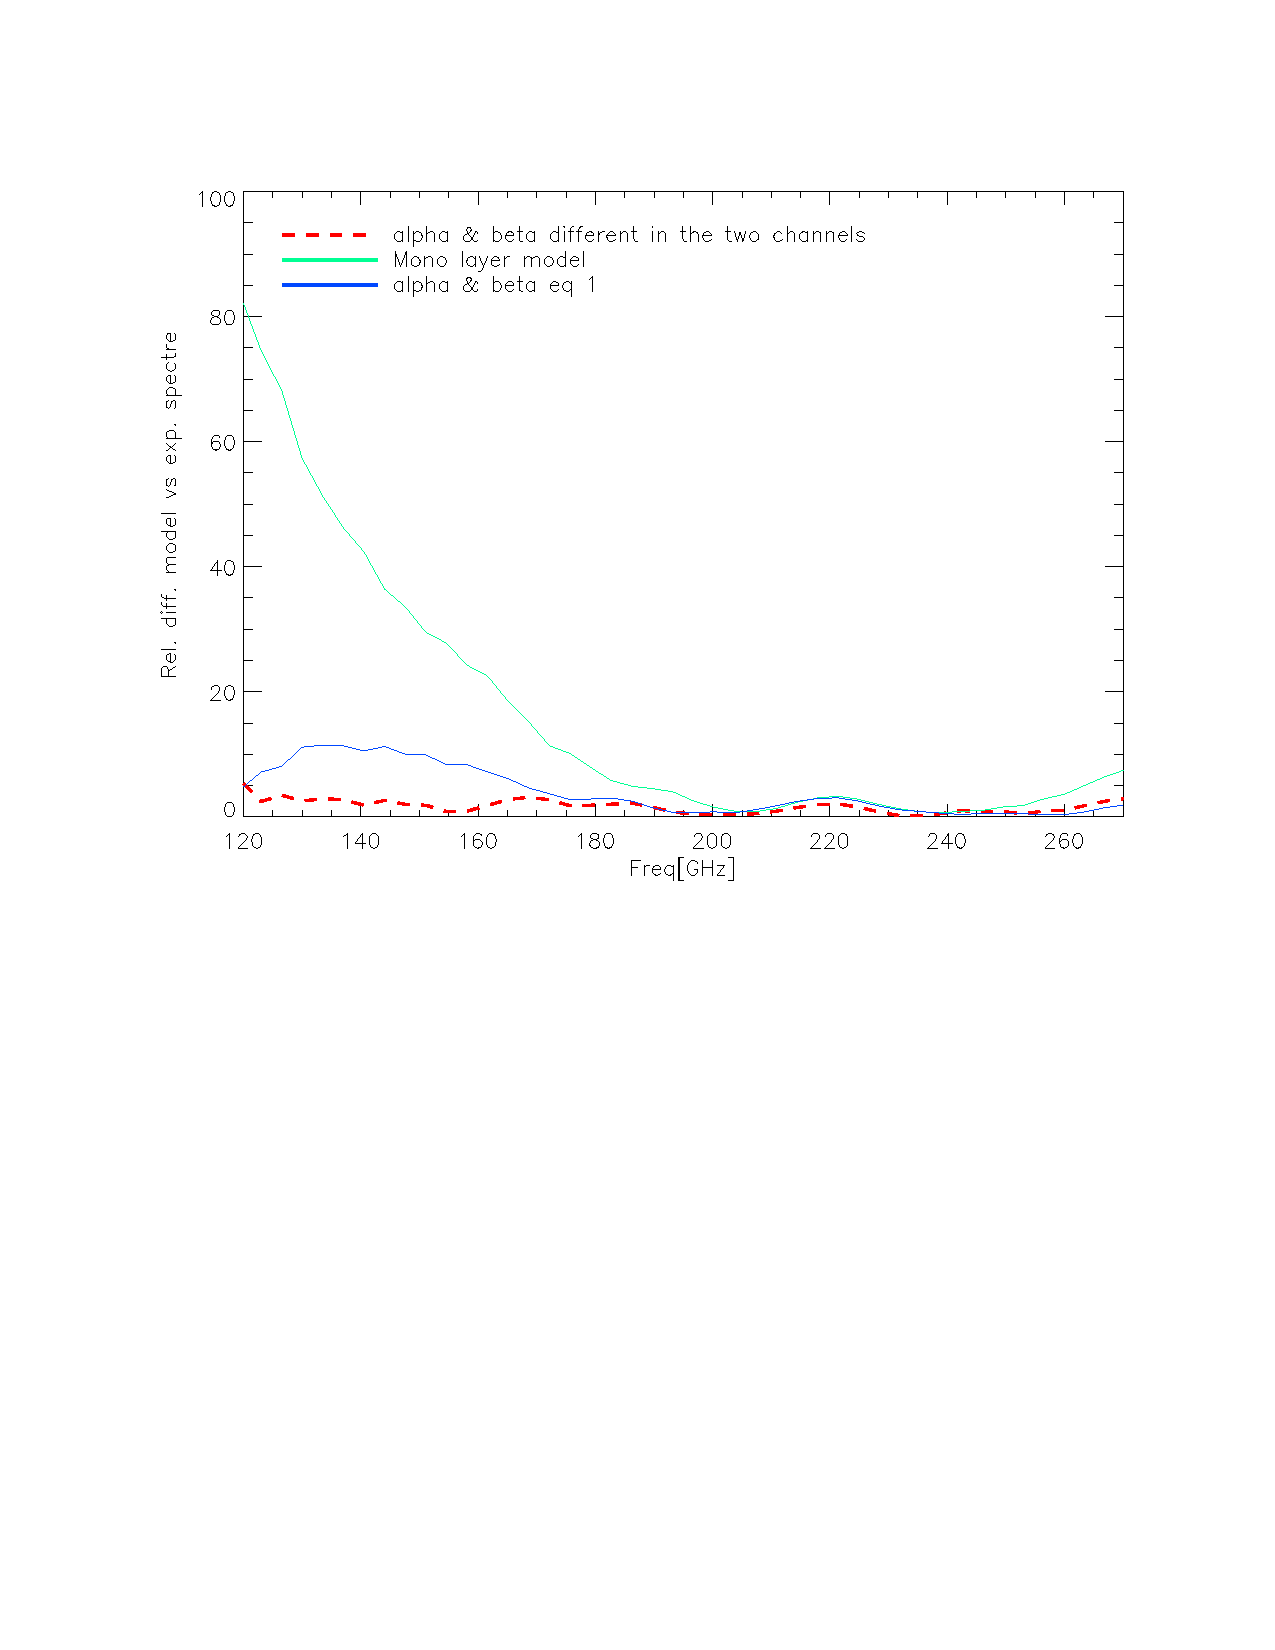
\includegraphics[height=13cm, width=16cm, trim=0cm 8cm 0cm 2cm, clip=true]{figures/Rel_diff_model}
	\caption{Deviation relative of the three model with the real observed spectrum, the y axis is done in \% }
	\label{fig:deviation}
\end{figure}

\begin{figure}
	\centering
	\includegraphics[height=7cm, width=16cm, trim=0cm 8cm 0cm 2cm, clip=true]{figures/Spectrum_HWP_mono}
	\hspace{2mm}
	\includegraphics[height=7cm,width=16cm, trim=0cm 8cm 0cm 2cm, clip=true]{figures/Spectrum_HWP_fixed}
	\includegraphics[height=7cm,width=16cm, trim=0cm 8cm 0cm 2cm, clip=true]{figures/Spectrum_HWP_optimized}
	
	\caption{On the top graph there is the model supposing an HWP mono-layer(green line). On the center it is plotted the model obtained using an achromatic half wave plate and fixing the transmission coefficient at 1. On the bottom the pale blue line dotted it's represents the model calculated with 2 different couples of transmission coefficients for 1mm and 2mm channel. The big red spectrum is the reference spectrum used for the model and the smaller one is the attenuated spectrum at relative angle of 25.2 {$\deg$} from the reference spectrum. }
	\label{fig:Spectra}
\end{figure}

\begin{table*} [t!]
	\begin{center}
		\scalebox{1}{%
			\begin{tabular}{cccccc}
				\hline
				& $\alpha$ & $\beta$ & Total transmission  \\
				\hline  \hline	
				channel 1.25mm & 1 & 0.98  &96\%  \\
				channel 2.05mm  &  0.98 &  0.92 &90\% \\
				\hline  \hline
			\end{tabular}
		}
	\end{center}
	\caption{Results of the HWP parameters} \label{tab1}
\end{table*}

\subsubsection{Polarization efficiency}
In the previous section we have chosen the model at which to refer, now we want to calculate the polarization efficiency integrated on the NIKA bands to estimate the loss in transmission.
From the equation of a real HWP (see the previous document 'NIKAPol') we can define the HWP polarisation efficiency as $\rho_{pol} = (1-2\gamma)/2$ where $\gamma = \frac{\alpha \beta \cos(\phi)}{\alpha^2 + \beta^2}$. By multiplying $\rho_{pol}$ to the NIKA intensity spectral bandpass we obtain the $Q-U$ spectra shown in figure \eqref{fig:pol_eff}.

\begin{figure}[!h]
	\centering
	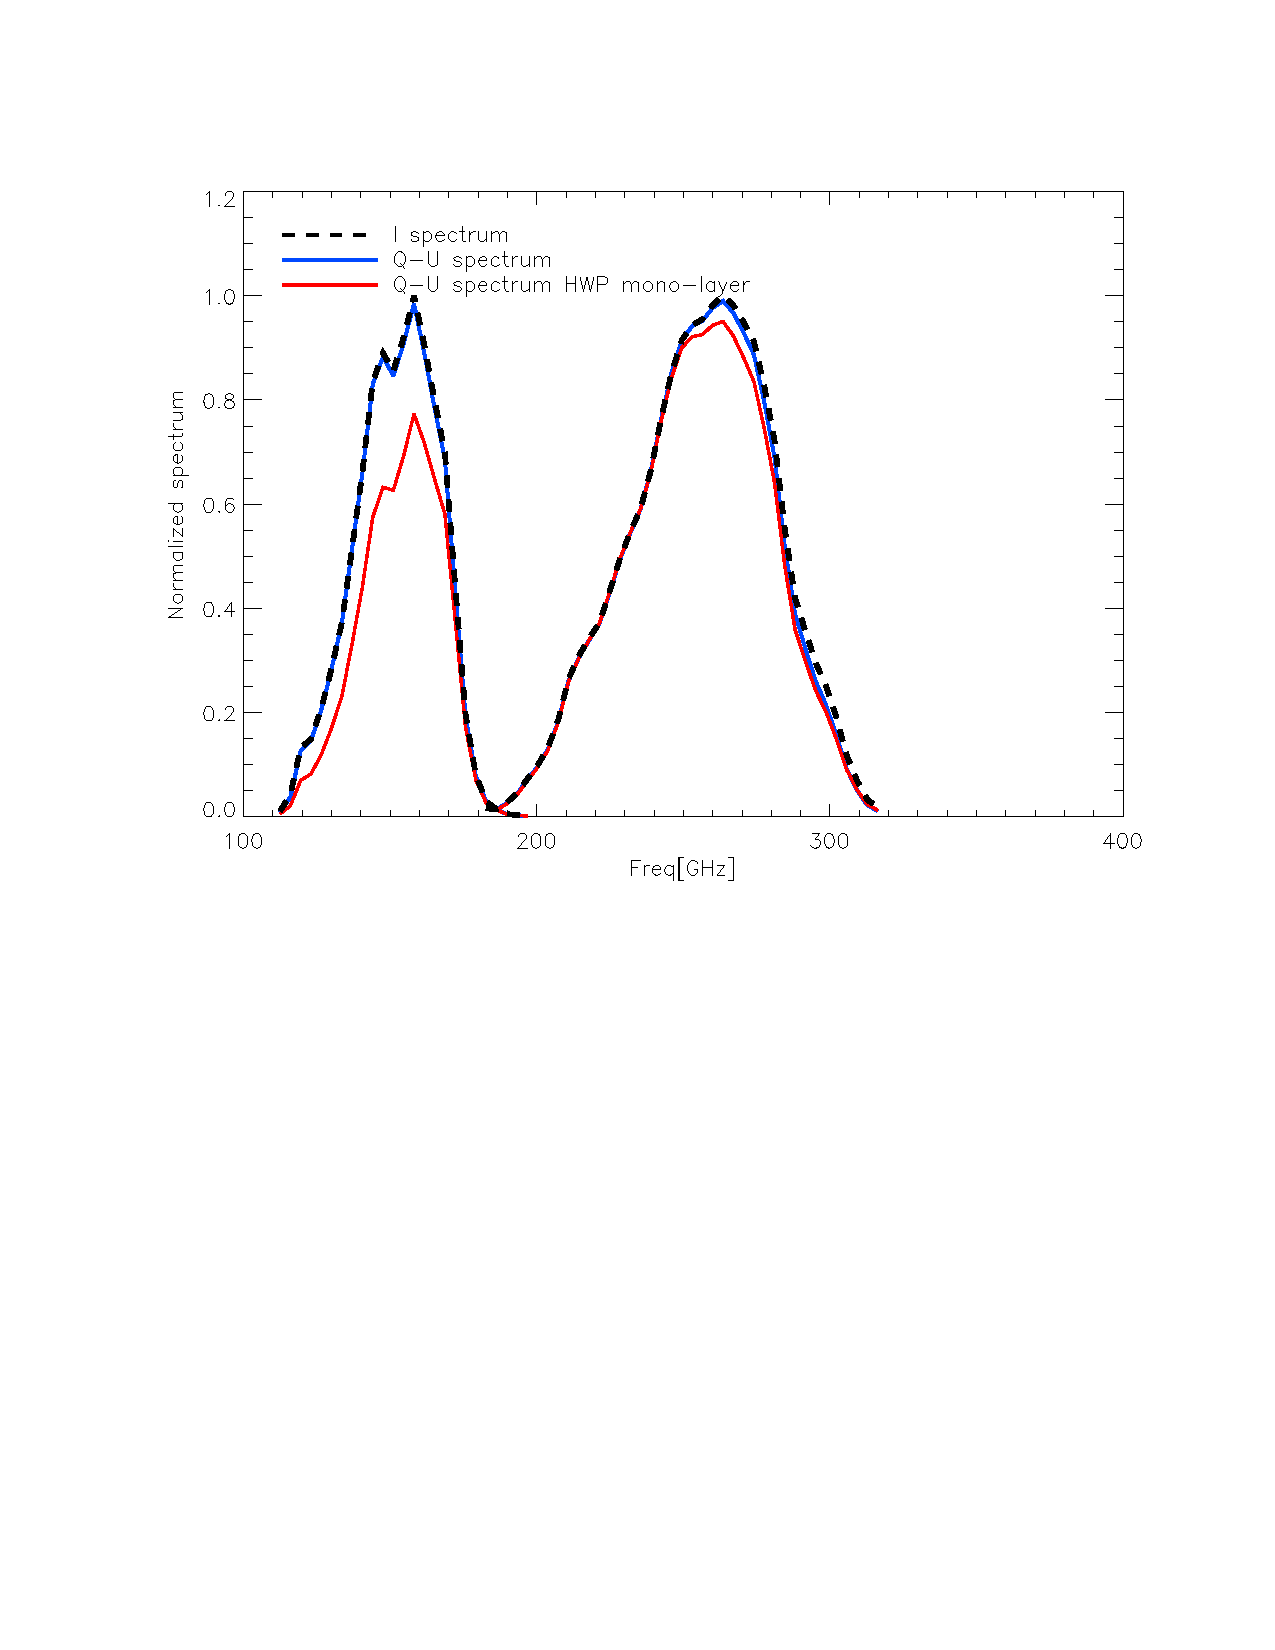
\includegraphics[height=13cm, width=16cm, trim=0cm 8cm 0cm 2cm, clip=true]{figures/Efficiency_Pol}
	\caption{Q-U spectrum of the AHWP model (blue) and mono layer HWP (red) and intensity spectrum (black dotted line) }
	\label{fig:pol_eff}
\end{figure}
\section{Conclusion}
From this analysis we can conclude that this new HWP has the maximum efficiency desirable in the broad band of NIKA.


\end{document}

